\documentclass[12pt,letterpaper]{article}
\usepackage{fullpage}
\usepackage[top=2cm, bottom=4cm, left=2cm, right=2cm]{geometry}
\usepackage{amsmath,amsthm,amsfonts,amssymb,amscd}
\usepackage{lastpage}
\usepackage{enumerate}
\usepackage{fancyhdr}
\usepackage{mathrsfs}
\usepackage{xcolor}
\usepackage{graphicx}
\usepackage{listings}
\usepackage{hyperref}
\usepackage{siunitx}
\usepackage{appendix}
\usepackage{caption}
\usepackage{subcaption}
\usepackage{multicol}
\usepackage{wrapfig}
\usepackage{esint}
\usepackage[utf8]{inputenc}
\usepackage[inline]{enumitem} %allows inline itemize or enumerate
\usepackage{pdfpages}


\hypersetup{%
  colorlinks=true,
  linkcolor=blue,
  linkbordercolor={0 0 1}
}
 
\renewcommand\lstlistingname{Algorithm}
\renewcommand\lstlistlistingname{Algorithms}
\def\lstlistingautorefname{Alg.}

\lstdefinestyle{Python}{
    language        = Python,
    frame           = lines, 
    basicstyle      = \tiny,
    keywordstyle    = \color{blue},
    stringstyle     = \color{green},
    commentstyle    = \color{orange}\ttfamily
}

\setlength{\parindent}{0.0in}
\setlength{\parskip}{0.1in}
\setlength{\tabcolsep}{6pt}

%Astronomical units
\DeclareSIUnit \parsec  {pc}
\DeclareSIUnit \year    {yr}

% Edit these as appropriate
% \newcommand\course{ASTRO 732}
% \newcommand\coursename{Computational Methods for Astrophysics}
\newcommand\course{ASTRO 645}
\newcommand\coursename{Astrophysical Dynamics}
\newcommand\hwnumber{4}
\newcommand\myname{Sandra Bustamante}  
%allows to number the last equation of align.
\newcommand\numberthis{\addtocounter{equation}{1}\tag{\theequation}}

\pagestyle{fancyplain}
\headheight 35pt
\lhead{\course \\ Homework \hwnumber}
\chead{\textbf{\Large Potential Theory}}
\rhead{\myname \\ Due October 29, 2019}
\lfoot{}
\cfoot{\coursename}
\rfoot{\small\thepage}
\headsep 1.5em

%redefines subsections to be letters instead of numbers so 1.a normal way is 1.1
% \arabic (1, 2, 3, ...)
% \alph (a, b, c, ...)
% \Alph (A, B, C, ...)
% \roman (i, ii, iii, ...)
% \Roman (I, II, III, ...)
\renewcommand\thesubsection{\thesection.\alph{subsection}}

%%%%%%%%%%%%%%%%%%%%%%%%%%%%%%%%%%%%%%%%%%%%%%%%%%%%%%%%%%%%%%%
%=====================BEGIN DOCUMENT===========================
%%%%%%%%%%%%%%%%%%%%%%%%%%%%%%%%%%%%%%%%%%%%%%%%%%%%%%%%%%%%%%%

\begin{document}
\twocolumn
\lstset{style=Python}

% textwidth is \the\textwidth \\
% column width is \the\columnwidth \\
% textheight is \the\textheight

\section{Turning points in spherical systems}

As we know, the apocenter $r_a$ and pericenter $r_p$ of an orbit in a spherical
stellar system is given by the roots of
\begin{equation}
    2(E -V(r))- \frac{J^2}{r^2}= 0.
\end{equation}

Prove that this equation has either zero or two roots assuming that
the orbit is bound $(E < 0)$ and the potential $V(r)$ is physically realizable (that is: it corresponds to a mass distribution with finite density).

[Hints: (i) Change variables to $u = 1/r$; (ii) use the Poisson equation
after taking the second derivative of equation (1).]
%\clearpage

\section{Symplectic integration.}

% Generalize your ODE program for integrating and plotting the equations of motion using the symplectic leapfrog integrator. I did not have
% time to discuss this algorithm in class today, but I’m attaching a brief
% introduction as an appendix to get you started. I will discuss this at the
% beginning of class next Thursday.
A symplectic integrator is an integrator that conserve phase-space volume and Poincar\' e invariants \cite{BinneyT_}

Explain Leapfrog 





%%%%%%%%%%%%%%%%%%%%%%%%%%%%%%%%%%%%%%%%%%%%%%%%%%%%%%%%%%%%%%%
%=========================SUBSECTION===========================
%%%%%%%%%%%%%%%%%%%%%%%%%%%%%%%%%%%%%%%%%%%%%%%%%%%%%%%%%%%%%%%
\subsection{}
% (a) As a test, use this integrate the pendulum equations of motion in
% all regimes:
% i. rotation,
% ii. libration,
% iii. near the unstable equilibrium
We can test our leapfrog code by integrating the equation of motion of the pendulum. 

The equation of motion of the pendulum is given by
\begin{equation}
    \Ddot{\theta}=-\sin\theta.
\end{equation}

We can determine 3 scenarios:
\begin{itemize}
    \item Rotation
    Rotation is when the total energy given by
    \begin{equation}
    E=\frac{1}{2}\Dot{\theta}^2+\left(1+\cos\theta\right)
    \end{equation}
    is bigger than the critical energy. The critical energy is 
    
    \item Libration
    \item Near Unstable Equilibrium
\end{itemize}

\begin{table}[]
    \centering
\begin{tabular}{lrr}
\toprule
{} &  $\theta$ &  $\dot{\theta}$ \\
\midrule
Rotation    &     -4.08 &             1.30 \\
Libration   &      0.50 &             0.00 \\
Near Uns Eq &      3.13 &             0.00 \\
\bottomrule
\end{tabular}

    \caption{Caption}
    \label{tab:PendulumIV}
\end{table}



%%%%%%%%%%%%%%%%%%%%%%%%%%%%%%%%%%%%%%%%%%%%%%%%%%%%%%%%%%%%%%%
%=========================SUBSECTION===========================
%%%%%%%%%%%%%%%%%%%%%%%%%%%%%%%%%%%%%%%%%%%%%%%%%%%%%%%%%%%%%%%
\subsection{}
(b) Demonstrate that the leapfrog integrator is second-order accurate
in the sense that errors in $\mathbf{q}$ and $\mathbf{p}$ after a timestep $h$ are $O(h^3)$.



%%%%%%%%%%%%%%%%%%%%%%%%%%%%%%%%%%%%%%%%%%%%%%%%%%%%%%%%%%%%%%%
%=========================SUBSECTION===========================
%%%%%%%%%%%%%%%%%%%%%%%%%%%%%%%%%%%%%%%%%%%%%%%%%%%%%%%%%%%%%%%
\subsection{}
(c) Compute the energy conservation for the trajectories in each regime
over about 10,000 orbital periods. Compare the energy conservation for RK4 and leapfrog.
%\clearpage

\section{Orbits in an axisymmetric potential}
Considering an axisymmetric potential for a simple model of a galaxian disk first proposed by Toomre (1964, ApJ):
\begin{equation}
    U(r) = -(1+r^2)^{-1/2},
\end{equation}

the equation of motion is given by
\begin{equation}
    F=-\frac{dU(r)}{dr}=-\frac{r}{(1+r^2)^{3/2}}.
\end{equation}

This is a differential equation that can be solved using leapfrog integration.

\begin{figure*}[h!]
    \centering
    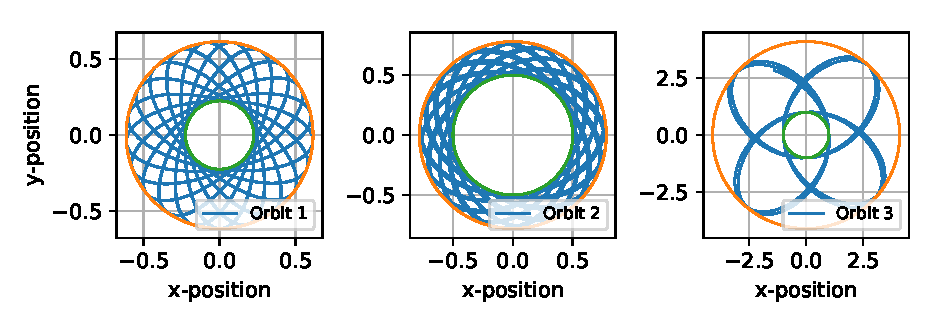
\includegraphics{CodeAndFigures/ToomrePotentialOrbits.pdf}
    \caption{Rosette Orbits using initial conditions of Left: $x=.3$, $y=0$, $v_x=.3$ and $v_y=.4$ Middle: $x=0$, $y=0.5$, $v_x=.6$ and $v_y=0$. Right:$x=1$, $y=0$, $v_x=0$ and $v_y=1$.}
    \label{fig:ToomreOrbits}
\end{figure*}

Using the initial values listed on table \ref{tab:ToomreOrbits}, we can calculate the orbits for each case. Figure \ref{fig:ToomreOrbits} shows that the orbits are not close but they precess. These types of orbits are called rosette orbits because of the shape or tube orbits because they have an inner and outer boundary.

\begin{table}
  \begin{center}
    \caption{Initial values used for calculating each rosette orbit using the Toomre potential.}
    \label{tab:ToomreOrbits}
    \pgfplotstabletypeset[
      
      col sep=comma, % the separator in our .csv file
      %display columns/0/.style={string type,column name={}},
%       display columns/0/.style={
% 		column name=Orbit, % name of first column
% 		%column type={S},string type
% 		},  % use siunitx for formatting
%       display columns/1/.style={column name=$x$,
% 		%column type={S},string type
% 		},
% 	  display columns/2/.style={column name=$y$,
% 		%column type={S},string type
% 		},
% 	  display columns/3/.style={column name=$v_x$,
% 		%column type={S},string type
% 		},
% 	 display columns/4/.style={column name=$v_y$,
% 		%column type={S},string type
% 		},
% 			 display columns/4/.style={
% 		column name=$v_y$,
% 		%column type={S},string type
% 		},
      every head row/.style={
		before row={\toprule}, % have a rule at top
		after row={
 			\midrule} % rule under units
 			},
	  every last row/.style={after row=\bottomrule}, % rule at bottom
    ]{CodeAndFigures/ToomreOrbitsData.csv} % filename/path to file
  \end{center}
\end{table}

These systems have two conserved quantities, the total energy $E_T$ and angular momentum $L$. Using the initial conditions, one can calculate the total energy of the system,
\begin{equation}
    E_T=K + U(r) = \frac{1}{2}v^2 + U(r)
\end{equation}
where U is the potential energy and K is the kinetic energy of the initial values, and the angular momentum by
\begin{equation}
    L=r^2\Dot{\theta}
\end{equation}
where 
\begin{align}
    r^2 = x^2 + y^2\\
    \Dot{\theta} = r \times \dot{r}\\
    \dot{r}^2 = v_x^2 + v_y^2
\end{align}.

Figure \ref{fig:conservedQuants} shows the total energy and the angular momentum of these rosette orbits are being conserved through time. 
\begin{figure*}[h!]
    \centering
    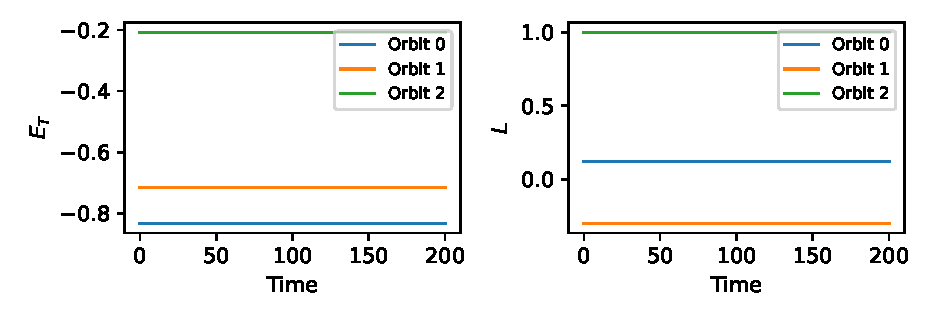
\includegraphics{CodeAndFigures/EnergyMomentumPlot.pdf}
    \caption{Left: Energy and Right: Angular Momentum of the rosette orbits in function with time.}
    \label{fig:conservedQuants}
\end{figure*}

The inner and outer radius of the orbits are found by finding the roots of
\begin{equation}
    E_T - U(r) - \frac{L^2}{r^2} = 0
    \label{eq:rootfunc}
\end{equation}

The bisect method was used to find the roots. The bisect methods finds the roots of a given function within a range of values to evaluate the function. The range for $r$ was determined by first plotting the equation \ref{eq:rootfunc} and determining visually were a sign change occurred. The value for inner and outer radius for each trial orbit is listed in table \ref{tab:ToomreOrbits} and is shown in Figure \ref{fig:ToomreOrbits} in orange and green. 





%\clearpage

\section{Non-axisymmetric orbits}

Finally, a more complicated non-axisymmetric case—two fixed point
masses—which has the potential:
\begin{equation}
    U(x,y) = -[(x-a)^2 +y^2]^{-1/2} -[(x+a)^2 +y^2]^{-1/2}.
\end{equation}

Although far from obvious, this potential can be separated in confocal
elliptical coordinates and put in a Staeckel form (as described in B\&T
and therefore has regular orbits. If the two point masses were in orbit
around each other, the orbits would not be regular. In other words, the
real three body problem has chaotic trajectories!
%%%%%%%%%%%%%%%%%%%%%%%%%%%%%%%%%%%%%%%%%%%%%%%%%%%%%%%%%%%%%%%
%=========================SUBSECTION===========================
%%%%%%%%%%%%%%%%%%%%%%%%%%%%%%%%%%%%%%%%%%%%%%%%%%%%%%%%%%%%%%%
\subsection{}
% (a) Again, pick some initial conditions and integrate the orbits. Just
% to be definite a = 1=2 (although the problem scales with a so you
% can choose value you wanted and get the same results).

The equations of motion for this potential are
\begin{align*}
    F&=-\nabla U(r) =-(\frac{\partial U(r)}{\partial x}+\frac{\partial U(r)}{\partial y}\\
    \Ddot{x}&=-\left[\frac{x-a}{(x-a)^2+y^2}+\frac{x+a}{(x+a)^2+y^2}\right] \\
    \Ddot{y}&=- \left[\frac{y}{(x-a)^2+y^2}+\frac{y}{(x+a)^2+y^2}\right]
\end{align*}

This can be evaluated using the initial conditions listed in table \ref{tab:NonAxisSymetric} and $a= \frac{1}{2}$.

\begin{table}[]
    \centering
    \begin{tabular}{lrrrrrr}
    \toprule \\
    Orbit &    x &    y &  $v_x$ &  $v_y$ &  $r_{inner}$ &  $r_{outer}$\\
    \midrule \\
    0 &  0.3 &  0.0 &  0.3 &  0.4 &    0.22 &   0.61 \\
    1 &  0.0 &  0.5 &  0.6 &  0.0 &    0.50 &   0.78 \\
    2 &  1.0 &  0.0 &  0.0 &  1.0 &    1.00 &   4.10 \\
    \bottomrule\\
    \end{tabular}
    \caption{Caption}
    \label{tab:my_label}
\end{table}

\begin{table}[]
    \centering
\begin{tabular}{lrrrrrr}
\toprule
{} &    x &    y &  $v_x$ &  $v_y$ &  $r_{inner}$ &  $r_{outer}$ \\
\midrule
Orbit 1 & 0.30 & 0.00 &   0.30 &   0.40 &         0.22 &         0.61 \\
Orbit 2 & 0.00 & 0.50 &   0.60 &   0.00 &         0.50 &         0.78 \\
Orbit 3 & 1.00 & 0.00 &   0.00 &   1.00 &         1.00 &         4.10 \\
\bottomrule
\end{tabular}

    \caption{Caption}
    \label{tab:my_label}
\end{table}

%%%%%%%%%%%%%%%%%%%%%%%%%%%%%%%%%%%%%%%%%%%%%%%%%%%%%%%%%%%%%%%
%=========================SUBSECTION===========================
%%%%%%%%%%%%%%%%%%%%%%%%%%%%%%%%%%%%%%%%%%%%%%%%%%%%%%%%%%%%%%%
\subsection{}
(b) There are two different kinds of orbits in this potential: tube orbits
and box orbits. Box orbits come arbitrarily close to the center of
force filling a closed area (similar to Lissajous figures). In fact,
there are two cases of box orbits here: those which come close to
one and those which come close to both centers of force. Find an
example of each case.
%%%%%%%%%%%%%%%%%%%%%%%%%%%%%%%%%%%%%%%%%%%%%%%%%%%%%%%%%%%%%%%
%=========================SUBSECTION===========================
%%%%%%%%%%%%%%%%%%%%%%%%%%%%%%%%%%%%%%%%%%%%%%%%%%%%%%%%%%%%%%%
\subsection{}
(c) Extra credit Investigate the relationship between conserved quantities and the envelope of the orbits. Report your findings.
Note: because the force is generated by two point masses, box orbits
will come arbitrarily close to one or both of the force centers. This
makes the solution numerically tricky. Consider using small error tolerances and/or small time steps . . .
%\clearpage

\section{Irregular orbits: Part 1}
Most often, one does not know the fraction of irregular orbits for particular density model. A very useful technique for both determining whether an orbit is regular or irregular and classifying the type of orbit
is the “surface of section” method. This is described in detail in B\&T section 3.2.2.

%%%%%%%%%%%%%%%%%%%%%%%%%%%%%%%%%%%%%%%%%%%%%%%%%%%%%%%%%%%%%%%
%=========================SUBSECTION===========================
%%%%%%%%%%%%%%%%%%%%%%%%%%%%%%%%%%%%%%%%%%%%%%%%%%%%%%%%%%%%%%%
\subsection{}
Adapt your ODE program to find the $x-\Dot{x}$ surface of section that
is, have your program plot with points the the values of $x$ and $\Dot{x}$
when $y = 0$ and $\Dot{y}> 0$.




%%%%%%%%%%%%%%%%%%%%%%%%%%%%%%%%%%%%%%%%%%%%%%%%%%%%%%%%%%%%%%%
%=========================SUBSECTION===========================
%%%%%%%%%%%%%%%%%%%%%%%%%%%%%%%%%%%%%%%%%%%%%%%%%%%%%%%%%%%%%%%
\subsection{}
Use your ODE program to find a tube orbit and a box orbit in the
potential given by B\&T equation 3-103 with $R_c = 0.14$, $q = 0.9$
and $v_c = 1$. (See Figure 3-8 for inspiration).




%%%%%%%%%%%%%%%%%%%%%%%%%%%%%%%%%%%%%%%%%%%%%%%%%%%%%%%%%%%%%%%
%=========================SUBSECTION===========================
%%%%%%%%%%%%%%%%%%%%%%%%%%%%%%%%%%%%%%%%%%%%%%%%%%%%%%%%%%%%%%%
\subsection{}
Now, plot the surface of section for these orbits. Note/discuss/explain
the differences. [We will explore the surface of sections for irregular orbits in a later PS.]

%\clearpage

\section{The Jacobi Integral}
% Recall the Jacobi integral discussed in class.
% \subsection{}
% Show that the Jacobi integral is a constant of the motion, i.e. $\frac{dE_j}{dt}=0$
The Jacobi integral in a rotating non axisymmetric potential is 
\begin{equation}
    E_J=\frac{1}{2}\Dot{x}^2 + \Phi(\mathbf{x}) - \frac{1}{2}\left|\mathbf{\Omega}_b \times \mathbf{x}\right|^2
\end{equation}
where $\mathbf{\Omega}_b$ is the constant rotation speed of the system whose direction is along the axis of rotation

It can be shown that it is a constant of motion by deriving with respect to time,
\begin{align*}
     \frac{dE_j}{dt}&=\frac{d}{dt}\left(\frac{1}{2}\Dot{x}^2 
     +\Phi(\mathbf{x}) 
     -\frac{1}{2}|\mathbf{\Omega}_b\times\mathbf{x}|^2\right)\\
     &=\Dot{x}\Ddot{x}+\Dot{x}\frac{d\Phi(\mathbf{x})}{d\mathbf{x}}-\frac{1}{2}\frac{d}{dt}\left(\Omega_b^2x^2 - (\mathbf{\Omega}_b\cdot\mathbf{x})^2\right)\\
     &=\Dot{x}\Ddot{x}+\Dot{x}\nabla\Phi(\mathbf{x})-\dot{\mathbf{x}}\Omega_b^2\mathbf{x}+ 
     \dot{\mathbf{x}}\mathbf{\Omega}_b(\mathbf{\Omega}_b\cdot\mathbf{x})\\
\end{align*}

From Hamilton's equation we can find that 
\begin{equation}
    \Ddot{x}=-\nabla\Phi(\mathbf{x})-2\mathbf{\Omega}_b\times\dot{\mathbf{x}}+\mathbf{\Omega}_b^2\mathbf{x}-\mathbf{\Omega}_b(\mathbf{\Omega}_b\cdot\mathbf{x})
\end{equation}
so substituting this into our equation and using the identity $A\cdot(B\times C)=B\cdot(C\times A)$ we get that
\begin{align*}
    \frac{dE_J}{dt}&=2\dot{\mathbf{x}}\left(\mathbf{\Omega}_b\times\dot{\mathbf{x}}\right)\\
    \frac{dE_j}{dt}&=2\mathbf{\Omega}_b\left(\dot{\mathbf{x}}\times\dot{\mathbf{x}}\right)
    \frac{dE_j}{dt}&=0
\end{align*}
Proving that the Jacobi integral is a constant of motion.

Additionally, knowing that the momentum in the underlying inertial frame can be described by $p=\dot{x}+\Omega_b\times x$,we can rewrite the Jacobi integral as
\begin{align*}
    E_J&=\frac{1}{2}\left(\mathbf{p}-\mathbf{\Omega}_b\times \mathbf{x}\right)^2 + \Phi(\mathbf{x}) - \frac{1}{2}\left|\mathbf{\Omega}_b \times \mathbf{x}\right|^2 \\
    &=\frac{1}{2}\left(p^2 -2\mathbf{p}\cdot(\mathbf{\Omega}_b\times\mathbf{x}\right)
    +\left|\mathbf{\Omega}_b \times \mathbf{x}\right|^2) + \Phi(\mathbf{x})\\
    &\quad \quad- \frac{1}{2}|\mathbf{\Omega}_b \times \mathbf{x}|^2 \\
    &=\frac{1}{2}p^2 -\mathbf{p}\cdot(\mathbf{\Omega}_b\times\mathbf{x})
    + \Phi(\mathbf{x})\\
    &=\frac{1}{2}p^2 -\mathbf{\Omega}_b\cdot(\mathbf{x}\times\mathbf{p})
    + \Phi(\mathbf{x})\\
    &=E-\mathbf{\Omega}_b\cdot\mathbf{L}
\end{align*}
where the total energy $E=\frac{1}{2}p^2+\Phi(\mathbf{x})$ and the angular momentum of the orbit $L=\mathbf{p}\times\mathbf{x}$.


% Show that the Jacobi integral for an orbit may be written as:
% \begin{equation}
%     E_J = E - \mathbf{\Omega}_p \cdot \mathbf{L}
% \end{equation}
% where $\mathbf{\Omega}_p$ is the constant rotation speed of the system whose direction is along the axis of rotation and $L$ is the angular momentum of the orbit.

\clearpage
%\newpage

%%%%%%%%%%%%%%%%%%%%%%%%%%%%%%%%%%%%%%%%%%%%%%%%%%%%%%%%%%%%%%%
%=====================Add Bibliography=========================
%%%%%%%%%%%%%%%%%%%%%%%%%%%%%%%%%%%%%%%%%%%%%%%%%%%%%%%%%%%%%%%

% \bibliographystyle{plain} % We choose the "plain" reference style
% %plain style sorts the reference list by alphabetical order of the first author’s last name.
% \bibliography{references} % Entries are in the "refs.bib" file

% % %\include{name} %name without extension. insert in new page

% \clearpage


%%%%%%%%%%%%%%%%%%%%%%%%%%%%%%%%%%%%%%%%%%%%%%%%%%%%%%%%%%%%%%%
%=====================Appendix=================================
%%%%%%%%%%%%%%%%%%%%%%%%%%%%%%%%%%%%%%%%%%%%%%%%%%%%%%%%%%%%%%%
% \appendix

% \lstset{caption={Astro732\_HW04P1.py}, style=Python}
% \section[]{Python code Problem 1} 
% \label{sec:CodeHw04p1}
% \lstset{label={Astro732Hw04P1.py}}
% \lstinputlisting[language=Python]{CodeAndFigures/Astro732_HW04P1.py}

% \clearpage

% \lstset{caption={Astro732\_Hw04P2.py}, style=Python}
% \section[]{Python code Problem 2} 
% \label{sec:CodeHw04p2}
% \lstset{label={Astro732HW04P2BestR0.py}}
% \lstinputlisting[language=Python]{CodeAndFigures/Astro732_HW04P2_BestR0.py}

% \clearpage

% \lstset{caption={Astro732\_Hw04p3.py}, style=Python}
% \section[]{Python code Problem 3} 
% \label{sec:CodeHw03p3}
% \lstset{label={Astro732Hw04p3.py}}
% \lstinputlisting[language=Python]{CodeAndFigures/Astro732_HW04P3.py}


\end{document}